\section{Einleitung}
Ziel des vorliegenden Versuchs ist es mit Hilfe des Faraday-Effektes die effektive
Masse von Elektronen des Halbleiters Galliumarsenid zu bestimmen.
\section{Theorie}
\subsection{Die effektive Masse}
Viele physikalische Effekte von Kristallen lassen sich durch die in Abbildung~\ref{fig:band}
dargestellte Bandstruktur von Festkörpern erklären.
\begin{figure}
  \centering
  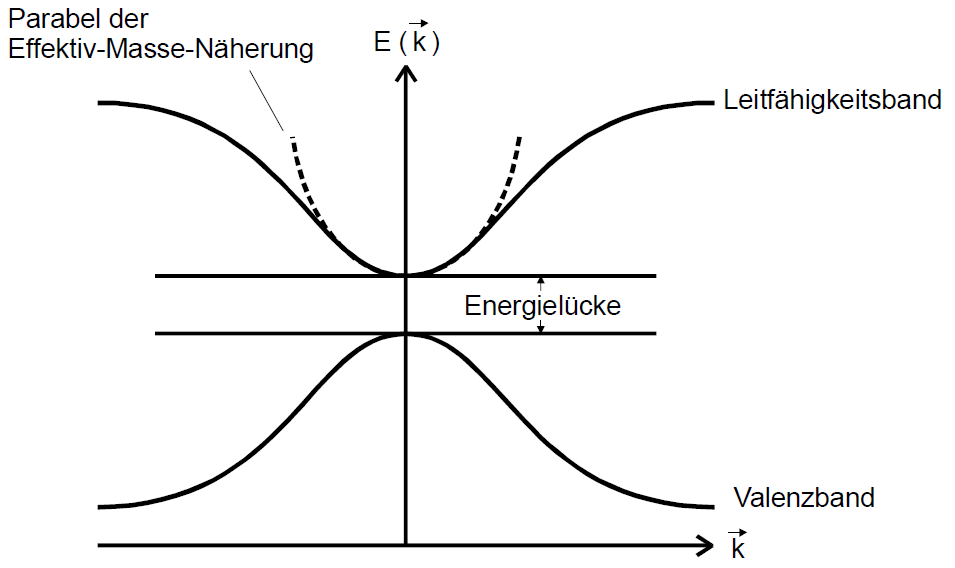
\includegraphics[width=0.6\textwidth]{graphics/band.png}
  \caption{Schematische Darstsellung der Bandstruktur eines Festkörpers \cite{anleitung}.}
  \label{fig:band}
\end{figure}
Die Form der Bandkante, welche die Elektronenenergie beschreibt, lässt sich durch die Funktion
\begin{equation}
  \epsilon = \epsilon(\vec{k}) = \frac{\hbar^2\vec{k}^2}{2m}
  \label{eqn:1}
\end{equation}
beschreiben, diese lässt sich an der Stelle $k=0$ um ihr Minimum entwickeln
\begin{equation}
  \epsilon(\vec{k}) = \epsilon(0) = \frac{1}{2}\sum_{i=1}^3 \left(\frac{\partial^2 \epsilon}{\partial k_i^2}\right)\bigg{\vert}_{x=0} k_i^2 + ...\;.
\end{equation}
Unter Verwendung der Defintion aus Formel~\eqref{eqn:1} lässt sich diese Gleichung zu einer Ellipsoidengleichung umstellen. Diese Gleichung beschreibt
im $\vec{k}$-Raum Flächen gleicher Energie. Bei Galliumarsenid sind diese Energieflächen auf Grund der hohen Kristallsymmetrie kugelförmig, sodass
sich ergibt:
\begin{equation}
  \epsilon(\vec{k}) = \epsilon(0) + \frac{\hbar^2k^2}{2m^{*}}\;.
\end{equation}
Das $m^*$ beschreibt dabei die effektive Masse eines Kristallelektrons mit
\begin{equation}
m^* = \frac{\hbar^2}{\left(\frac{\partial^2 \epsilon}{\partial k_i^2}\right)\bigg{\vert}_{x=0}}.
\end{equation}
Die effektive Masse beinhaltet dabei schon das periodische Kristallpotential $V(\vec{r}+\vec{g})$, sodass die Elektronen als
freie Teilchen beschreiben werden und sich der Hamilton vereinfacht zu
\begin{equation*}
  \mathscr{H} = \frac{\hbar^2}{2m^*}\Delta\;.
\end{equation*}

\subsection{Rotation der Polarisationsebene}
Die Polarisationsebene eines linear polarisierten Lichtstrahles kann beim Transmittieren in einen Kristall aus optisch aktivem Medium gedreht
werden. Da dies beim Eintreffen und beim Austreten aus dem Kristall passiert, wird dieses Phänomen zirkulare Doppelbrechung genannt. Dieser
Effekt kann bei optisch inaktiven Materialien durch das Anlegen eines äußeren Magnetfeldes erreicht werden.
Bei diesem Vorgang muss zwischen links- und rechtspolarisiertem Licht unterschieden werden, da sich die beiden Anteile mit unterschiedlichen
Phasengeschwindigkeiten bewegen. Eine elektromagnetische Welle, die sich in $z$-Richtung ausbreitet, wird daher durch
\begin{equation}
  E(z) = \frac{1}{2}(E_\text{L}(z) + E_\text{R}(z))
\end{equation}
dargestellt, wobei $k_\text{L} \neq k_\text{R}$ gilt.
Nachdem der Lichtstrahl den Kristall der Länge L durchlaufen hat, wurde die Polarisationsebene um den Winkel $\vartheta$ gedreht. Dieser
lässt sich durch die Wellenzahlvektoren $k_i$ beschreiben und mit Hilfe der Phasengeschwindigkeit $v_\text{Ph} = \frac{\omega}{k}$ und dem Brechungsindex
$n = \frac{c}{v_\text{Ph}}$ umschreiben zu:
\begin{equation}
  \vartheta = \frac{L}{2}(k_\text{R} - k_\text{L}) = \frac{L\omega}{2}(\frac{1}{v_\text{PhR}} - \frac{1}{v_\text{PhL}}) = \frac{L\omega}{2c}(n_\text{R} - n_\text{L})
\end{equation}
Durch die Wechselwirkung der Bandelektronen mit den Atomrümpfen der Gitteratome entstehen bei der Doppelbrechung induzierte Dipolmomente,
die ihrerseits wieder pro Volumen eine Polarisation erzeugen.
\begin{equation}
  \vec{P} = \epsilon_0\chi\vec{E}
\end{equation}
Für doppeltbrechende Materie wird die elektrische Suszeptibilität $\chi$ durch den Tensor:
\begin{equation}
  (\chi)=
  \begin{pmatrix}
  \chi_\text{xx} & i\chi_\text{xy} & 0\\
    -i\chi_\text{xy} & \chi_\text{yy} & 0\\
    0 & 0 & \chi_\text{zz}
  \end{pmatrix}
\end{equation}
beschrieben. Durch Anwendung der Wellengleichung lässt sich der Drehwinkel auf:
\begin{equation}
  \vartheta = \frac{L\omega}{2cn}\chi_\text{xy}
\end{equation}
zurückführen. Die Suszeptibilitätskomponente $\chi_\text{xy}$ wird durch die Bewegungsgleichung~\eqref{eqn:bew} bestimmt. Dabei werden Dämpfungseffekte
vernachlässigt und durch das hohe $\omega$ werden nur Verschiebungspolarisationen $\vec{P} \propto \vec{r}$ betrachtet.
\begin{equation}
   m \frac{\text{d}^2\vec{r}}{\text{dt}^2} + K\vec{r} = -e_0\vec{E}(r) - e_0\frac{\text{d}\vec{r}}{\text{dt}}
   \label{eqn:bew}
\end{equation}
Aus ihr geht hervor, dass die beiden Nichtdiagonalelemente komplex konjugiert sind und sich der Drehwinkel $\vartheta$ in Abhängigkeit der
Wellenlänge $\lambda$ schreiben lässt:
\begin{equation}
  \vartheta(\lambda) = \frac{2\pi^2e_0^3c}{\epsilon_0 m^2\lambda^2\omega_0^4}\frac{NBL}{n}\;.
\end{equation}
Im Grenzfall freier Ladungsträger geht $\omega_0 \shortrightarrow 0$ und somit ergibt sich für den Drehwinkel von Kristallelektronen
\begin{equation}
  \vartheta_{frei} = \frac{e_0^3\lambda^2}{8\pi^2\epsilon_0c^3}\frac{NBL}{n m^{*2}}\;.
  \label{eq:frei}
\end{equation}
